\documentclass[letterpaper]{article}

\usepackage[english]{babel}
\usepackage[utf8]{inputenc}
\usepackage{amsmath}
\usepackage{graphicx}
\usepackage[colorinlistoftodos]{todonotes}

\title{Heat Transfer in a Ring \\ Spring 2014, 22.559}

\author{Josh Bevan}

\date{\today}

\begin{document}
\maketitle

\section{Problem Statement}
\begin{figure}
\centering
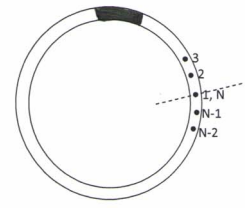
\includegraphics[width=0.4\textwidth]{Ring.PNG}
\caption{\label{fig:ring}Schematic of heated ring with coincident nodes at joint.}
\end{figure}

\begin{figure}[!htb]
\centering
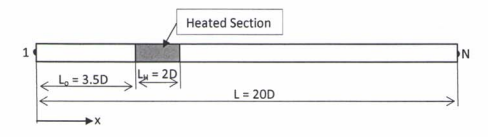
\includegraphics[width=0.6\textwidth]{Unrolled.PNG}
\caption{\label{fig:unrolled}"Unrolled" ring, coincident nodes at either end.}
\end{figure}

A ring has a heated section with a constant heat flux and is cooled convectively (see Fig \ref{fig:ring}). Determine the temperature distribution for steady-state conditions. If the ring is "unrolled" the problem becomes 1D with periodic boundary conditions (see Fig \ref{fig:unrolled}). The unrolled ring can be discretized and if nodes are placed at both ends, they will be coincident.

\textit{Calculate the temperature distribution for 21 nodes if the Biot number for this system is Bi=0.05.}

\section{Theoretical Approach}
For a differential ring section control volume \(dx\) thick the energy balance can be found to be in accordance with \eqref{energybalance}

\begin{equation}\label{energybalance}
\frac{\partial^2 T}{\partial x^2} - \frac{hp}{kA}(T-T_\infty) + \frac{q}{kA} = 0
\end{equation}

Using the dimensionless quantities \eqref{theta} and \eqref{eta}, substituting them into \eqref{energybalance}, simplifying algebraically, changing \(\theta(x) \to \theta(\eta(x))\), and applying the chain rule yields \eqref{dimlessbalance}

\begin{equation}\label{eta}
\eta = \frac{x}{D}
\end{equation}
\begin{equation}\label{theta}
\theta = \frac{T-T_\infty}{\frac{q'D^2}{kA}}
\end{equation}
\begin{equation}\label{dimlessbalance}
\frac{\partial^2 \theta(\eta)}{\partial x^2} - 4Bi\theta(\eta) = -1
\end{equation}

In the region of the ring where a constant heat flux is generated \eqref{dimlessbalance} holds true, in sections free of heat generation the RHS is instead 0.

\section{Discretization}
Integrating across the control volume and taking the numerical derivative yields a differential operator that takes the same form as the 2nd order Taylor expansion for the derivative of the form
\begin{equation}\label{2nddiff}
\frac{\partial^2 \theta(\eta)}{\partial x^2} \approx \frac{\theta(\eta_{i-1})-2\theta(\eta_i)+\theta(\eta_{i+1})}{\Delta x^2}
\end{equation}

\section{Application}
Applying the discretization in \eqref{2nddiff} to \eqref{dimlessbalance} generates a linear equation for each node in the domain. There are $N$ unknowns and $N$ linearly independent equations for the $N+1$ nodes (as nodes $N+1$ and $1$ are coincident). This system of equations can be represented as a linear system $\mathbf{Ax=F}$ with $\mathbf{A}$ representing the LHS of \eqref{dimlessbalance}, $\mathbf{x}$ the solution vector and $\mathbf{F}$ the RHS forcing of \eqref{dimlessbalance}. \\*

$\mathbf{A} = \frac{1}{\Delta x^2}
 \begin{pmatrix}
  -2 & 1 & 0 & 0 & 0 & \cdots & 1 & 0 \\
  1 & -2 & 1 & 0 & 0 & \cdots & 0 & 0 \\
  0 & 1 & -2 & 1 & 0 & \cdots & 0 & 0 \\
  \vdots  & \vdots & \vdots & \ddots & \ddots & \ddots & 0 & 0\\
  0 & 0 & \cdots & 0 & 1 & -2 & 1 & 0\\
  0 & 0 & \cdots & 0 & 0 & 1 & -2 & 1\\
  0 & 1 & \cdots & 0 & 0 & 0 & 1 & -2
 \end{pmatrix}
 -(4Bi)\mathbf{I}$
 
 Note the jumps necessary at the enpoints of the domain to skip the coincident node. This linear system can be very compactly represented in Matlab and the solution vector solved for. $\mathbf{A}$ takes a form very similiar to a Toeplitz matrix, if the coincident node is omitted it takes the same form. Non-zero entries for $\mathbf{F}$ are entered at those control volumes within the heated region of the ring.
 
\begin{figure}
\centerline{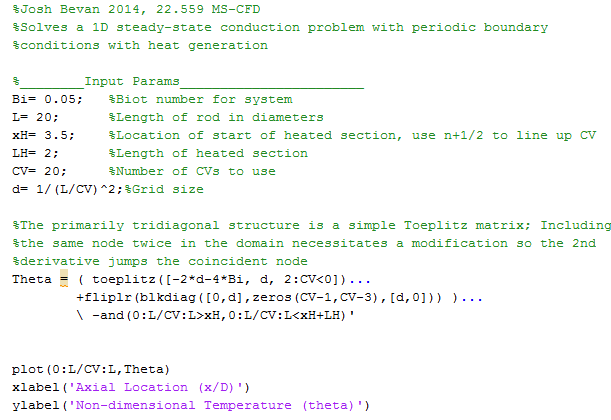
\includegraphics[width=1.2\textwidth]{PeriodicRingCode.PNG}}
\end{figure}

\section{Results}
The value of the dimensionless temperature at each grid point is tabulated in \ref{fig:ResultTable}. Additionally it is plotted in \ref{fig:graph} along with the solution for 2000 nodes. It is remarkable how well the results agree; the only discrepancy occurs in the heated region of the ring. There are only two nodes here and they are symmetrically placed about the centerline of the heated region so they are at the same temperature. This results in the flat region which fails to resolve any change in temperature between the nodes. More broadly speaking any region where a maxima or minima occurs nearly in between two nodes will inadequately capture the change.

\begin{figure}[b]
\centerline{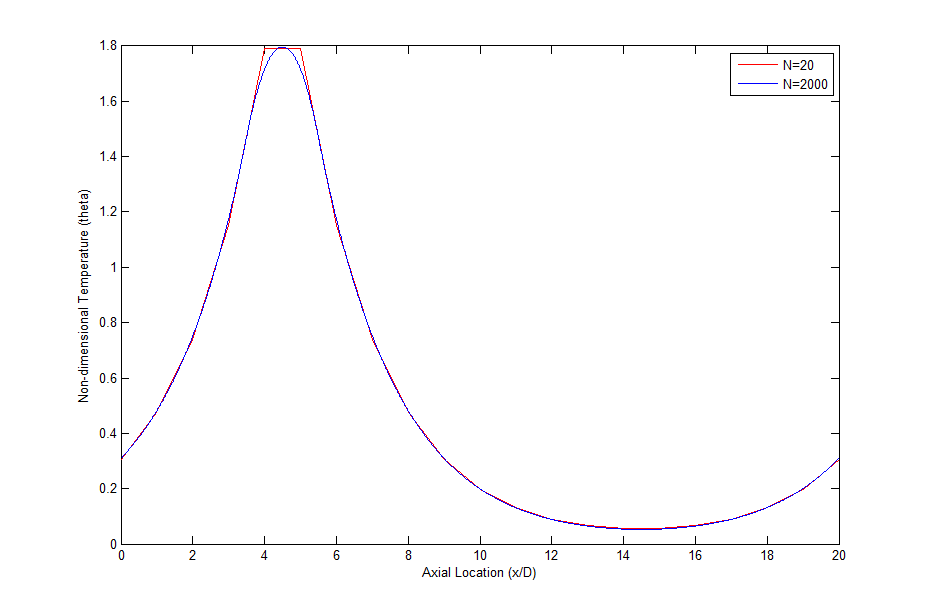
\includegraphics[width=1.5\textwidth]{N20-2000.png}}
\caption{\label{fig:graph}Temperature distribution for 20 and 2000 CVs.}
\end{figure}

\begin{table}
\centering
\begin{tabular}{l|c|c|r}
	Node & $\theta$ & Node & $\theta$\\
	\hline
	1	& 0.3062 & 12  & 0.1307\\
	2   & 0.4750 & 13  & 0.0890\\
	3   & 0.7388 & 14  & 0.0652\\
	4   & 1.1503 & 15  & 0.0543\\
	5   & 1.7919 & 16  & 0.0543\\
	6   & 1.7919 & 17  & 0.0652\\
	7   & 1.1503 & 18  & 0.0890\\
	8   & 0.7388 & 19  & 0.1307\\
	9   & 0.4750 & 20  & 0.1986\\
	10  & 0.3062 & 21  & 0.3062\\
	11  & 0.1986\\
\end{tabular}
\caption{\label{fig:ResultTable}Dimensionless temperature at each node.}
\end{table}    

\end{document}